\documentclass[11pt]{article}
\usepackage[margin=1in]{geometry}
\usepackage[T1]{fontenc}
\usepackage{lmodern}
\usepackage{graphicx}
\usepackage{booktabs}
\usepackage{caption}
\usepackage{subcaption}
\usepackage{xcolor}
\usepackage{tikz}
\usetikzlibrary{positioning,arrows.meta,shapes.geometric,fit}
\usepackage[hidelinks]{hyperref}
\usepackage{titlesec}
\usepackage{enumitem}
\setlist{nosep,leftmargin=1.4em}
\emergencystretch=2em

\renewcommand{\thesection}{\Roman{section}}
\titleformat{\section}{\normalfont\large\bfseries}{\thesection.}{0.5em}{}
\titlespacing*{\section}{0pt}{1.0ex}{0.5ex}

% Marks text still to be filled in before submission.
\newcommand{\todo}[1]{\textcolor{red}{[TODO: #1]}}
\newcommand{\tbd}{\textcolor{red}{?}}

\title{\vspace{-3em}Concept-to-Animation: LLM-Generated Manim Explainer Videos\\[0.2em]
\large CSE 434 Midterm Check-in Report}
\author{Jonah Femiani \and Koray Bayram}
\date{November 13, 2026}

\begin{document}
\maketitle
\vspace{-1.5em}
\begin{center}
\small
\textbf{Team:} Concept-to-Animation \quad
\textbf{Roles:} \emph{Jonah} --- baseline pipeline (LLM client, planner, code generation, render harness, logging, ablation runner), repair and layout loops, analysis, demo.
\emph{Koray} --- few-shot curation, RAG corpus and retriever, narration.
\emph{Both} --- human evaluation and reports.
\end{center}

% ---------------------------------------------------------------------------
\section{Project Overview}

Given a short description of a math or CS concept (e.g.\ ``binary search''), our system writes a short explainer video in the style of 3Blue1Brown by having an LLM plan a storyboard and then write Manim Community Edition (ManimCE) code for each scene.
LLM-written animation code fails in two characteristic ways: it calls \emph{hallucinated or outdated Manim APIs} (the code crashes), and it produces \emph{bad layouts} (objects overlap or leave the frame).
Our research question is: \textbf{which generative techniques make LLM-written animation code render reliably and look clear?}
We answer it with a cumulative ablation that starts from a zero-shot baseline and adds one technique at a time: error-driven self-repair, few-shot examples, retrieval-augmented generation (RAG) over the ManimCE docs, and a layout-repair loop driven by a bounding-box checker.
This connects directly to course topics on prompting, in-context learning, RAG, iterative self-refinement, and LLM code generation.

% ---------------------------------------------------------------------------
\section{Dataset}

\textbf{Concepts.} We curated 6 concepts in three difficulty tiers of two each, chosen by how directly the idea maps to pictures:
\emph{concrete} (Pythagorean theorem, derivative as slope),
\emph{structural} (matrix multiplication, binary search), and
\emph{abstract} (recursion, Big-O notation).
Each has a one-sentence prompt; the tiers let us ask whether performance drops as concepts get less visual.

\textbf{Storyboards.} For each concept the planner produces a storyboard of 3--4 scenes (20 scenes in total), each with a title, a visual description and narration.
Storyboards are validated against a schema and cached, so every condition generates code for exactly the same scenes and only the code-generation step differs.
All 6 were produced in one batch on 2026-11-10 by the same model.

\textbf{Retrieval corpus (planned):} the ManimCE docs and example gallery (MIT license), pinned to our render version (v0.22.1), chunked and embedded for RAG.

\textbf{Ethics.} The data contains no personal information. The main risk is that a fluent, polished video can teach \emph{wrong} math; render success does not catch this, so we add human ratings of mathematical correctness. Generated videos will be labeled as AI-generated.

% ---------------------------------------------------------------------------
\section{Methods}

Figure~\ref{fig:system} shows the current system (v1).
A \textbf{planner} turns the concept into a storyboard. A \textbf{code generator} writes one ManimCE \texttt{Scene} subclass per storyboard scene; its prompt states the pinned Manim version, forbids the older ManimGL library, and gives the frame bounds ($x\in[-7.1,7.1]$, $y\in[-4,4]$).
Post-processing is deliberately minimal (extract the code block, rename the class) so it cannot silently fix the errors we are measuring.
Each scene is \textbf{rendered} in a separate subprocess with a 120\,s timeout; we check that the expected video file was actually written, because Manim exits successfully even when the named scene does not exist.
Failures are \textbf{classified} from the traceback into \texttt{hallucinated\_api}, \texttt{bad\_signature}, \texttt{latex}, \texttt{timeout}, \texttt{syntax} or \texttt{other}.
Manim's \texttt{Mobject} invents any \texttt{get\_*} method on demand, so a hallucinated call like \texttt{axes.get\_secant\_line(\ldots)} surfaces as a \texttt{TypeError}; our classifier still labels it a hallucinated API.
Every attempt is logged as one JSONL line (tokens, latency, error, code path), and responses are cached so reruns cost nothing.

\begin{figure}[t]
\centering
\resizebox{\textwidth}{!}{%
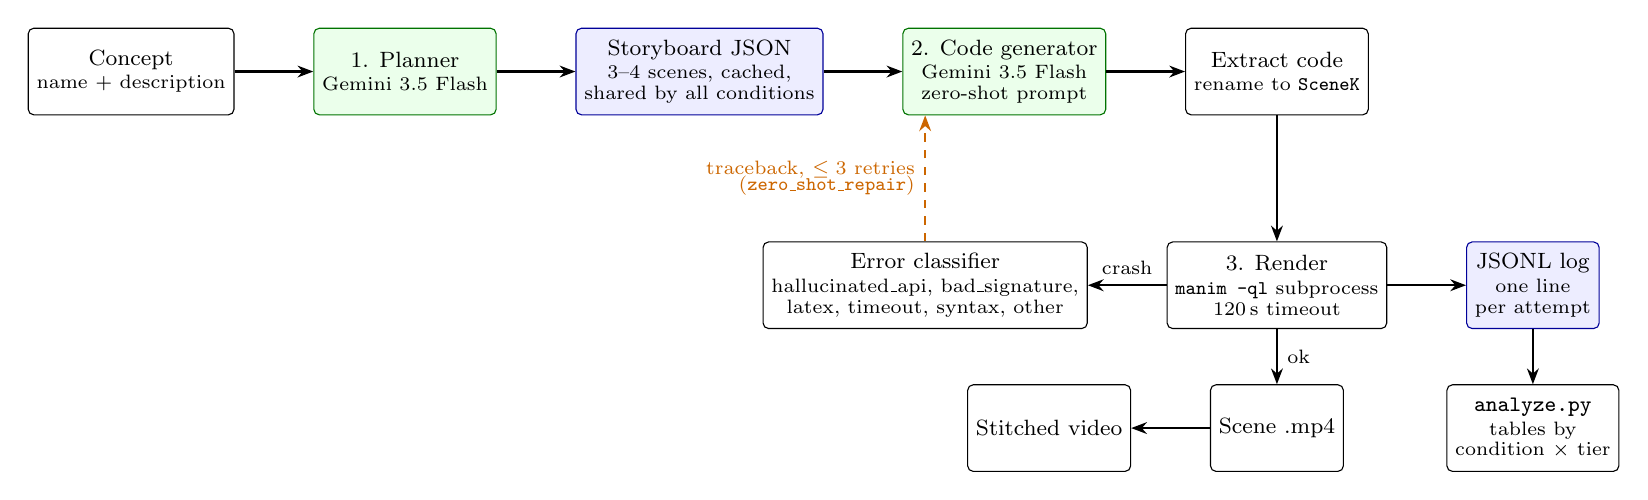
\begin{tikzpicture}[
  node distance=5mm and 10mm,
  box/.style={draw, rounded corners=2pt, align=center, font=\footnotesize, minimum height=11mm, inner sep=3pt},
  store/.style={box, fill=blue!7, draw=blue!60!black},
  llm/.style={box, fill=green!8, draw=green!45!black},
  arr/.style={-{Stealth[length=2mm]}, thick},
  repairarr/.style={arr, dashed, draw=orange!80!black}
]
\node[box] (c) {Concept\\[-1pt]\scriptsize name + description};
\node[llm, right=of c] (p) {1. Planner\\[-1pt]\scriptsize Gemini 3.5 Flash};
\node[store, right=of p] (sb) {Storyboard JSON\\[-1pt]\scriptsize 3--4 scenes, cached,\\[-2pt]\scriptsize shared by all conditions};
\node[llm, right=of sb] (g) {2. Code generator\\[-1pt]\scriptsize Gemini 3.5 Flash\\[-2pt]\scriptsize zero-shot prompt};
\node[box, right=of g] (x) {Extract code\\[-1pt]\scriptsize rename to \texttt{SceneK}};
\node[box, below=16mm of x] (r) {3. Render\\[-1pt]\scriptsize \texttt{manim -ql} subprocess\\[-2pt]\scriptsize 120\,s timeout};
\node[box, left=of r] (e) {Error classifier\\[-1pt]\scriptsize hallucinated\_api, bad\_signature,\\[-2pt]\scriptsize latex, timeout, syntax, other};
\node[box, below=7mm of r] (v) {Scene .mp4};
\node[box, left=of v] (s) {Stitched video};
\node[store, right=of r] (l) {JSONL log\\[-1pt]\scriptsize one line\\[-2pt]\scriptsize per attempt};
\node[box, below=7mm of l] (a) {\texttt{analyze.py}\\[-1pt]\scriptsize tables by\\[-2pt]\scriptsize condition $\times$ tier};

\draw[arr] (c) -- (p);
\draw[arr] (p) -- (sb);
\draw[arr] (sb) -- (g);
\draw[arr] (g) -- (x);
\draw[arr] (x) -- (r);
\draw[arr] (r) -- node[above, font=\scriptsize]{crash} (e);
\draw[arr] (r) -- node[right, font=\scriptsize]{ok} (v);
\draw[arr] (v) -- (s);
\draw[arr] (r) -- (l);
\draw[arr] (l) -- (a);
\draw[repairarr] (e.north) -- node[left, align=right, font=\scriptsize, text=orange!80!black]{traceback, $\le 3$ retries\\[-2pt](\texttt{zero\_shot\_repair})} (e.north |- g.south);
\end{tikzpicture}}
\caption{System design v1. Green: LLM calls; blue: stored artifacts. Solid path: the zero-shot baseline. Dashed: the error-repair loop (\texttt{zero\_shot\_repair}), which feeds the traceback back to the code generator. Few-shot, RAG and layout repair will attach to the code generator later.}
\label{fig:system}
\end{figure}

\textbf{Experimental design.} The full study is a cumulative ablation over six conditions: \texttt{zero\_shot}, \texttt{zero\_shot\_repair}, \texttt{few\_shot}, \texttt{rag}, \texttt{rag\_repair} and \texttt{rag\_repair\_layout}. Temperature is fixed at 0.2, conditions without repair get exactly one render attempt, and repair conditions get up to three extra attempts. Per-scene metrics, aggregated by condition and tier: render success, first-try success, repair iterations, layout-defect rate, error types, and two human scores (failed scene $=0$, so they reflect the whole pipeline).

\textbf{Changes since the proposal} (approved by Dr.~Zhang).
(1)~\emph{Gemini 3.5 Flash instead of GPT + an open model:} we tried Qwen2.5-Coder (7B and 3B, 4-bit via Ollama), but its Manim code was too poor to make the comparison informative; open models stay available behind our LLM interface.
(2)~\emph{No LangChain:} plain Python lets us log every prompt, reply and token count exactly.
(3)~\emph{6 concepts instead of 40,} so every condition can be run and every video hand-rated.

% ---------------------------------------------------------------------------
\section{Preliminary Results}

Table~\ref{tab:results} reports both conditions on all 20 scenes. Zero-shot renders 70\% of scenes, roughly evenly across tiers; error-driven repair raises this to \textbf{100\%}, needing 0.45 extra attempts per scene on average. Structural scenes (matrix grids, arrays) needed the most help (0.83 repairs per scene), so at this stage difficulty tracks how much layout code a scene needs, not how abstract the concept is. Repair costs about 2.3$\times$ the tokens per scene (4.3k vs.\ 1.9k). One caveat: every call reported its model as \texttt{gemini-3.6-flash}, so \texttt{gemini-3.5-flash} is an alias; we log the version to detect drift.

\begin{table}[h]
\centering
\footnotesize
\setlength{\tabcolsep}{5pt}
\begin{tabular}{lccccc}
\toprule
 & \multicolumn{3}{c}{Automatic} & \multicolumn{2}{c}{Human (0--5; failed scene $=0$)} \\
\cmidrule(lr){2-4}\cmidrule(lr){5-6}
Condition & Render success & First-try success & Avg.\ repairs & Correctness & Clarity \\
\midrule
\texttt{zero\_shot} & 70\% (14/20) & 70\% & -- & \tbd & \tbd \\
\quad concrete (7) & 71\% (5/7) & 71\% & -- & \tbd & \tbd \\
\quad structural (6) & 67\% (4/6) & 67\% & -- & \tbd & \tbd \\
\quad abstract (7) & 71\% (5/7) & 71\% & -- & \tbd & \tbd \\
\addlinespace
\texttt{zero\_shot\_repair} & \textbf{100\% (20/20)} & 70\% & 0.45 & \tbd & \tbd \\
\quad concrete (7) & 100\% (7/7) & 71\% & 0.29 & \tbd & \tbd \\
\quad structural (6) & 100\% (6/6) & 67\% & 0.83 & \tbd & \tbd \\
\quad abstract (7) & 100\% (7/7) & 71\% & 0.29 & \tbd & \tbd \\
\bottomrule
\end{tabular}
\caption{Gemini 3.5 Flash, all 20 scenes (scenes per tier in parentheses). For \texttt{zero\_shot\_repair}, render minus first-try success is what repair adds; avg.\ repairs is over scenes that eventually rendered. Human scores: mean of both raters over all 20 scenes; rendered scenes rated 1--5 blind to condition, failed scenes scored 0.}
\label{tab:results}
\end{table}
% Partial run (2026-11-10, 11/20 scenes, superseded by the full run): 72.7% (8/11) overall;
% concrete 5/7, structural 2/3, abstract 1/1.

\begin{figure}[h]
\centering
\hfill\begin{subfigure}{0.31\textwidth}
  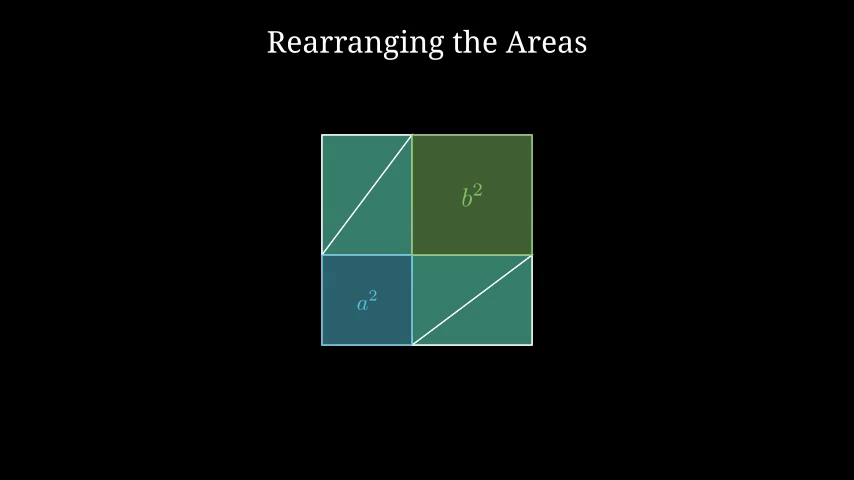
\includegraphics[width=\linewidth]{figures/pythagorean_s3.png}
  \caption{Pythagorean theorem, scene 3 (rendered).}
\end{subfigure}\hfill
\begin{subfigure}{0.31\textwidth}
  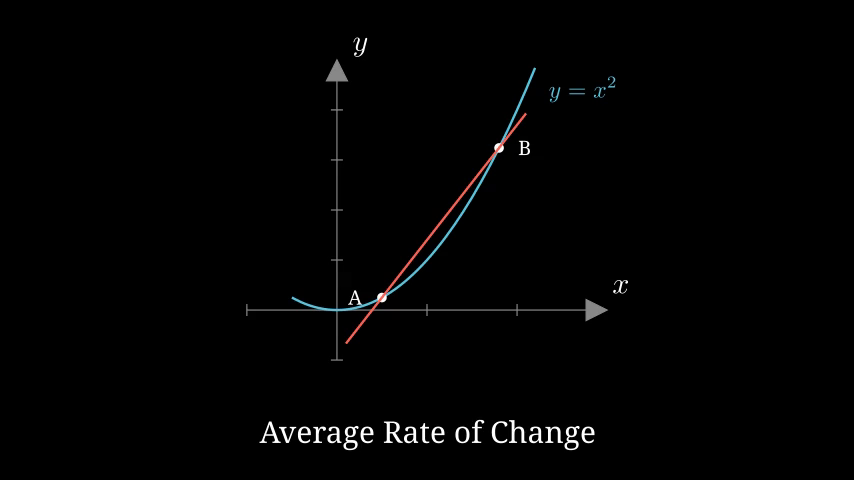
\includegraphics[width=\linewidth]{figures/derivative_s1.png}
  \caption{Derivative as slope, scene 1 (rendered).}
\end{subfigure}\hfill\null
\caption{Final frames from two zero-shot scenes that rendered on the first try.}
\label{fig:frames}
\end{figure}

\textbf{Qualitative examples.} \emph{Success:} all four Pythagorean-theorem scenes rendered first try; scene~3 (Fig.~\ref{fig:frames}a) rearranges four triangles in an $(a+b)$ square to expose $a^2$ and $b^2$, a clean, correct version of the classic proof. \emph{Contrasting failure:} for the derivative, scene~1 (Fig.~\ref{fig:frames}b) correctly draws a secant through two points on $y=x^2$, but scenes 2 and 3, which must \emph{animate} the secant approaching the tangent, both crashed zero-shot: the model called convenience methods (\texttt{axes.get\_secant\_line}, \texttt{get\_tangent\_line}) that sound right but do not exist in ManimCE. Given the traceback, repair replaced each with a small helper method that computes the line itself, and both scenes rendered on the second attempt. Repair is not always one step: in matrix multiplication scene~2, fixing an invalid keyword exposed an undefined color \texttt{CYAN} (which the model then defined itself), then a LaTeX error; it rendered on the fourth and last attempt.

\textbf{Error types.} All six zero-shot failures are API misuse, never syntax: three \texttt{bad\_signature} (e.g.\ \texttt{grid\_stroke\_width}), two \texttt{hallucinated\_api}, and one misused \texttt{TransformMatchingTex}. Each error names the bad call, which is why repair works so well and what RAG over the real docs should prevent up front.

\textbf{Human ratings.} \todo{mean correctness and clarity per condition (failed scenes $=0$), inter-rater agreement, and what the ratings show that render success does not.}

% ---------------------------------------------------------------------------
\section{Next Steps}

\begin{itemize}
  \item \textbf{Few-shot and RAG} (Koray): 3--5 curated modern ManimCE example scenes, and a retriever over the pinned ManimCE docs checked on whether it returns the right classes (e.g.\ \texttt{Axes.plot} for graphs).
  \item \textbf{Layout repair:} snapshot bounding boxes after each animation, flag off-frame objects and unintended overlaps, and describe them to the LLM in plain language. Since repair already reaches 100\% render success, clarity and correctness are now the metrics that can separate the remaining conditions.
  \item \textbf{Evaluation and demo:} the full six-condition ablation by tier, cost per condition, a success/failure gallery, gTTS narration and a type-a-concept web demo.
\end{itemize}

\textbf{Open questions for feedback.} Are 20 scenes enough to separate conditions? Is a bounding-box check a fair proxy for clarity, or should clarity rest on human ratings alone? Should we add leave-one-out rows to check the ablation's stacking order?

\end{document}
